\documentclass[12pt]{article}
\usepackage[utf8]{inputenc}

% Default fixed font does not support bold face
\DeclareFixedFont{\ttb}{T1}{txtt}{bx}{n}{12} % for bold
\DeclareFixedFont{\ttm}{T1}{txtt}{m}{n}{12}  % for normal

% Custom colors
\usepackage{color}
\definecolor{deepblue}{rgb}{0,0,0.5}
\definecolor{deepred}{rgb}{0.6,0,0}
\definecolor{deepgreen}{rgb}{0,0.5,0}
\setlength{\parskip}{2pt}%
\setlength{\parindent}{0pt}%
\usepackage{enumitem, amsmath, graphicx, wrapfig, float, nccmath, verbatim, fancyvrb, geometry, changepage, listings}
\usepackage[export]{adjustbox}
\newcommand\pythonstyle{\lstset{
		language=Python,
		basicstyle=\ttm,
		otherkeywords={self},             % Add keywords here
		keywordstyle=\ttb\color{deepblue},
		emph={MyClass,__init__},          % Custom highlighting
		emphstyle=\ttb\color{deepred},    % Custom highlighting style
		stringstyle=\color{deepgreen},
		frame=tb,                         % Any extra options here
		showstringspaces=false            % 
}}


% Python environment
\lstnewenvironment{python}[1][]
{
	\pythonstyle
	\lstset{#1}
}
{}

% Python for external files
\newcommand\pythonexternal[2][]{{
		\pythonstyle
		\lstinputlisting[#1]{#2}}}

% Python for inline
\newcommand\pythoninline[1]{{\pythonstyle\lstinline!#1!}}
\title{%
	ECE-471 Selected Topics in Machine Learning \\
	Prof. Curro \\
	Midterm Project}
\author{Evan Bubniak, Zhang Jinhan}
\begin{document}
\maketitle

\section{Summary}

The purpose of this project is to reproduce a subset of experimental results from the paper \textit{Understanding deep learning requires rethinking generalization} (Zhang et al. 2016), specifically Figure 1, which plots the average loss against the number of training steps for various types of example/label corruption. The experiment demonstrates that various kinds of label corruption do not prevent complete memorization of the training dataset, as long as the model is sufficiently large, and that the convergence of the model to 100\% accuracy is shifted by only a constant factor when data corruption is introduced.

The paper does not specify certain hyperparameters, specifically number of epochs and batch size. This proved problematic as the interplay between these two variables affects the number of steps needed to converge. Furthermore, although five models are specified as part of the CIFAR-10 experimental set-up, it is not specified if only one model was used to generate Figure 1, or if multiple model results were averaged together.

We conducted several tests to reconstruct and verify the experimental setup. Specifically, we rebuilt each of the five models described in Table 1 of the original paper: two minified InceptionV3 models respectively with and without batch normalization, a minified AlexNet, and two multi-layer perceptions with 512 units and, respectively, one and three hideen layers. These models were defined in Keras and are stated in the appendix.

The experimental setup involved, in total, the training and analysis of 25 models, corresponding to five models each trained on five datasets. Training was performed on the KAHAN server.

Our results show strong agreement with Figure 1 for the first model specified, the minified InceptionV3, and strong divergence in all other models. The two models are displayed side-by-side. 

\section{Results}

\begin{figure}[H]
	\centering
	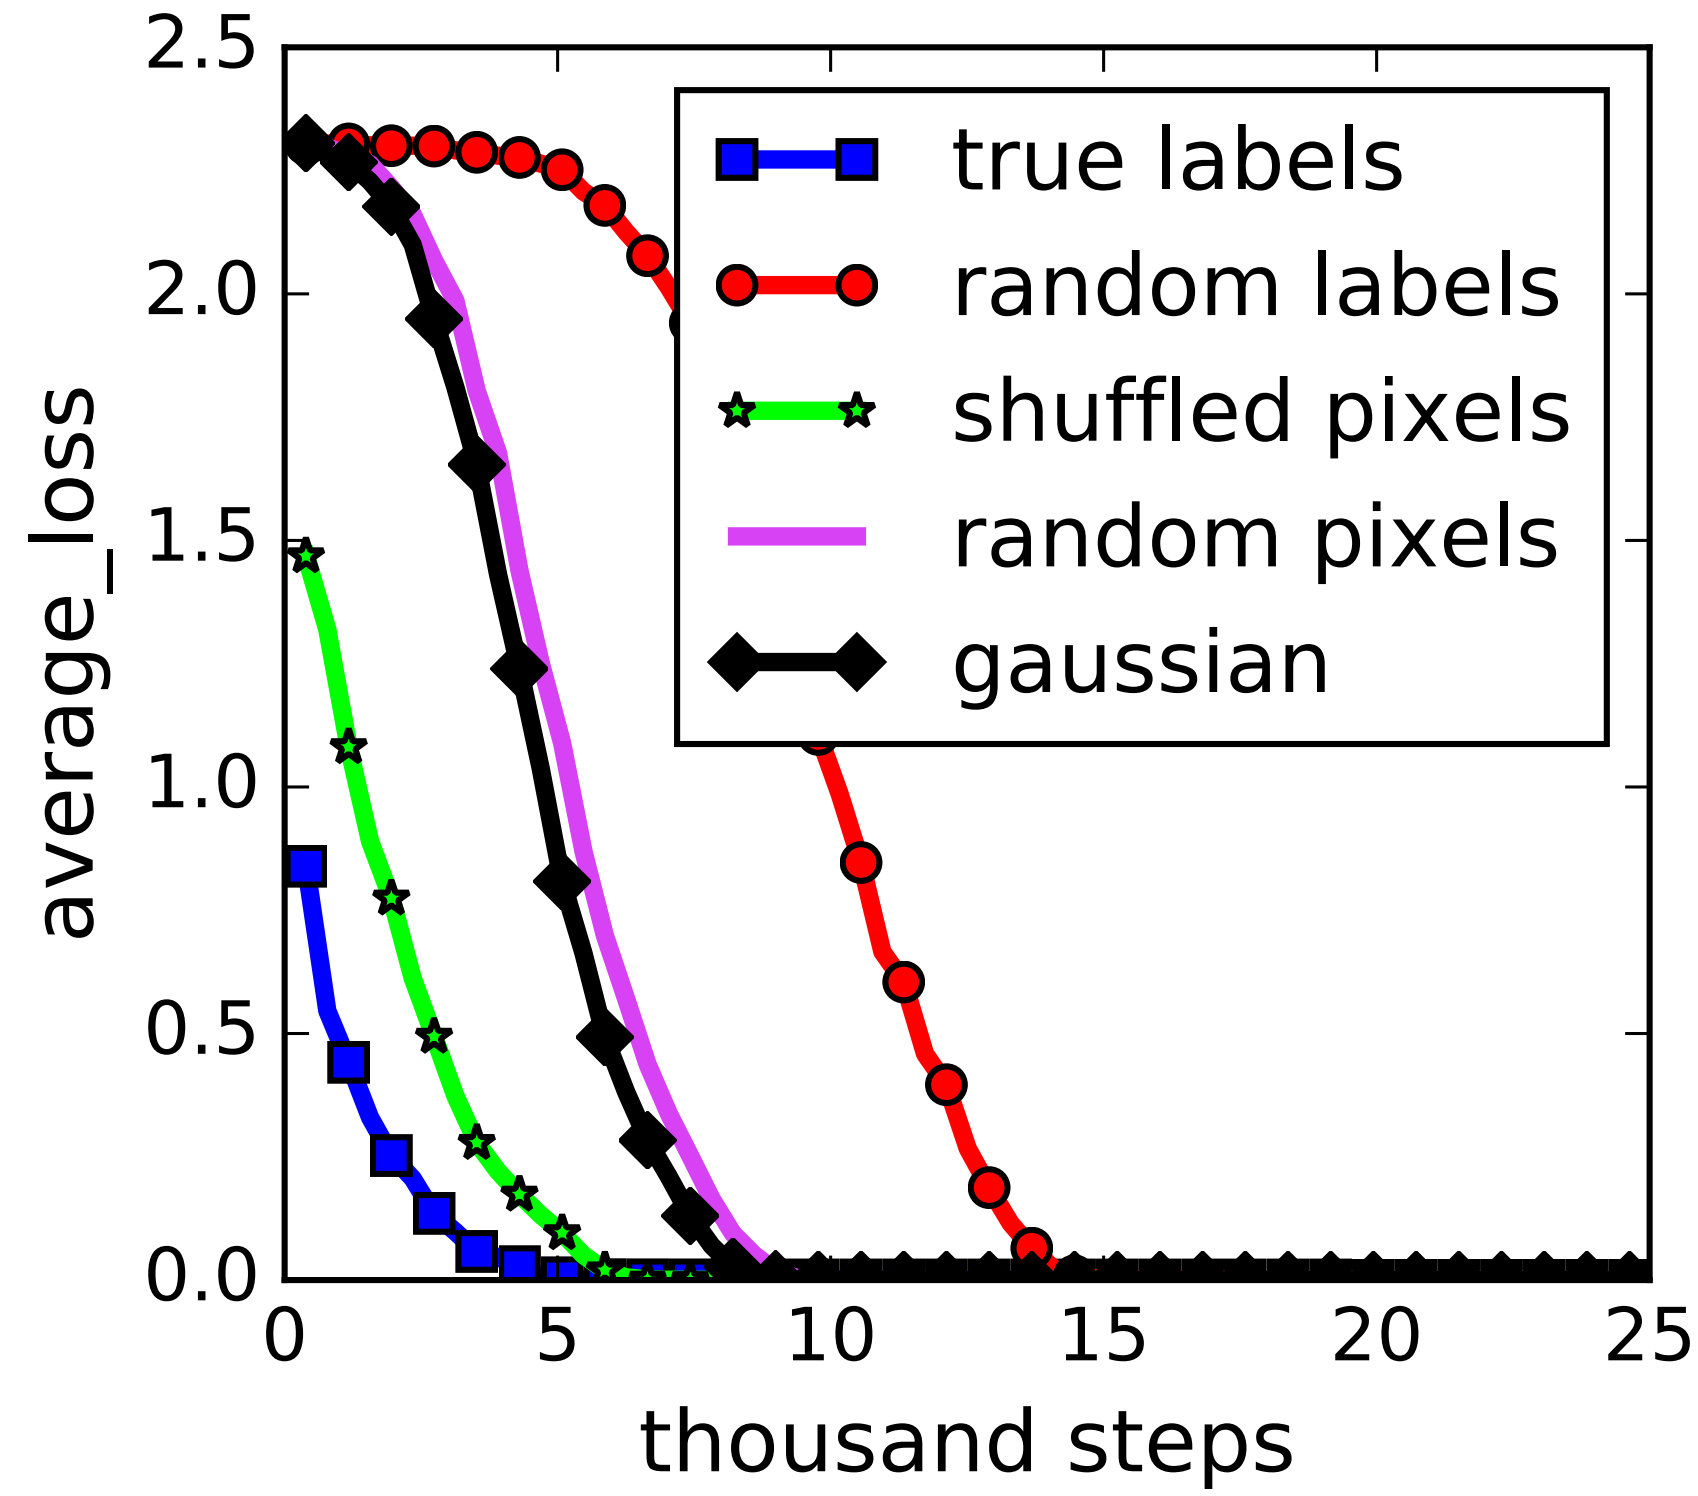
\includegraphics[width=0.75\textwidth]{fig.png}
	\caption{Juxtaposition of the noisy data points, the noiseless sinewave they are based on, and the manifold of the stochastic gradient descent regression model.}
\end{figure}

\begin{figure}[H]
	\centering
	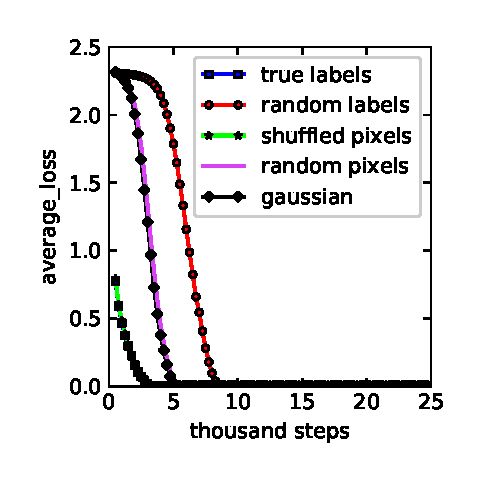
\includegraphics[width=0.75\textwidth]{MiniInceptionV3.eps}
	\caption{A plot of each of the basis functions, with the weights and intercept removed.}
\end{figure}

\clearpage
\begin{adjustwidth}{-50pt}{0pt}

\section{Appendix}
\subsection{Main Loop}
\pythonexternal{C:/Users/evanb/Documents/deeplearning/midterm/main.py}

\subsection{Data Preprocessing}
\pythonexternal{C:/Users/evanb/Documents/deeplearning/midterm/utils/preprocess_data.py}

\subsection{Data Corruption}
\pythonexternal{C:/Users/evanb/Documents/deeplearning/midterm/utils/data_corruption.py}

\subsection{Model Definitions}
\pythonexternal{C:/Users/evanb/Documents/deeplearning/midterm/utils/Models.py}
\end{adjustwidth}

\subsection{Matplotlib configuation}
\pythonexternal{C:/Users/evanb/Documents/deeplearning/midterm/plot_results.py}

\end{document}